\chapter{Hardware}
\section{Logic of submodule electronics}

All the logic of the submodule is shown in the figure \ref{fig:submodule_logic}.

\begin{figure}[H]
\includegraphics[width=1.05\linewidth]{logic}
\caption{Logic diagram of submodule electronics.}
\label{fig:submodule_logic}
\end{figure}

MEMS driver works independently from other modules, controlling only MEMS mirror. SiPM and Laser driver are joint by trigger signal. Laser driver utilize for shooting of laser diode, SiPM board generating high voltage for SiPM, performs readout and amplification of SiPM signal and measuring time delay between outgoing and return impulse by TDC chip.
Power supply for all components is +5V. Each components are described in detail below.

\subsection{Laser driver logic}
It is very easy to operate a laser diode, in addition to power supply (+5V) of a laser driver, we just need provide LH (Logical High, 3.3V for here) to the Enable input and clock signal with desirable frequency $f$ to the Trigger input, after that Laser driver repeats electrical 40A pulses with 10ns width for Laser diode.

\begin{figure}[H]
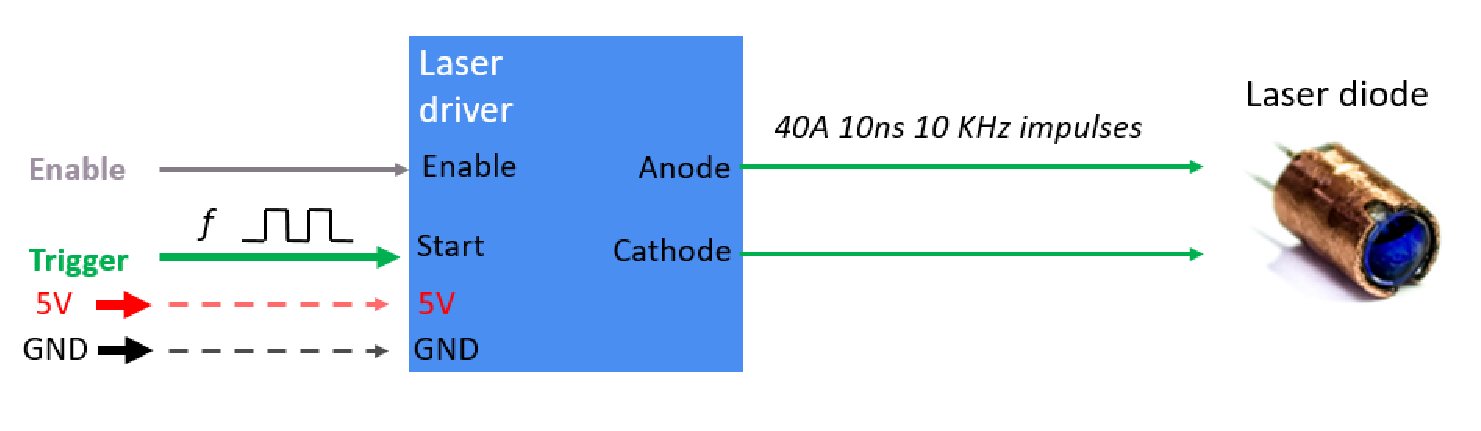
\includegraphics[width=1\linewidth]{ld_logic}
\caption{Logic diagram of laser driver.}
\label{fig:real_submodule}
\end{figure}

\subsection{MEMS driver logic}

MEMS driver board has a power (+5V) and control (SPI) input which are used for the control of MEMS mirror via SPI commands to 16-bit DAC, which produces a high-voltage (160V) 4-channel signal (X+, X-, Y+, Y-). 
We used 16-bit DAC with 20MHz SPI speed. 
Filter clocks input is used for set LPF cutoff frequency, to avoid high frequency which can induce resonance and damage of the mirror.


\begin{figure}[H]
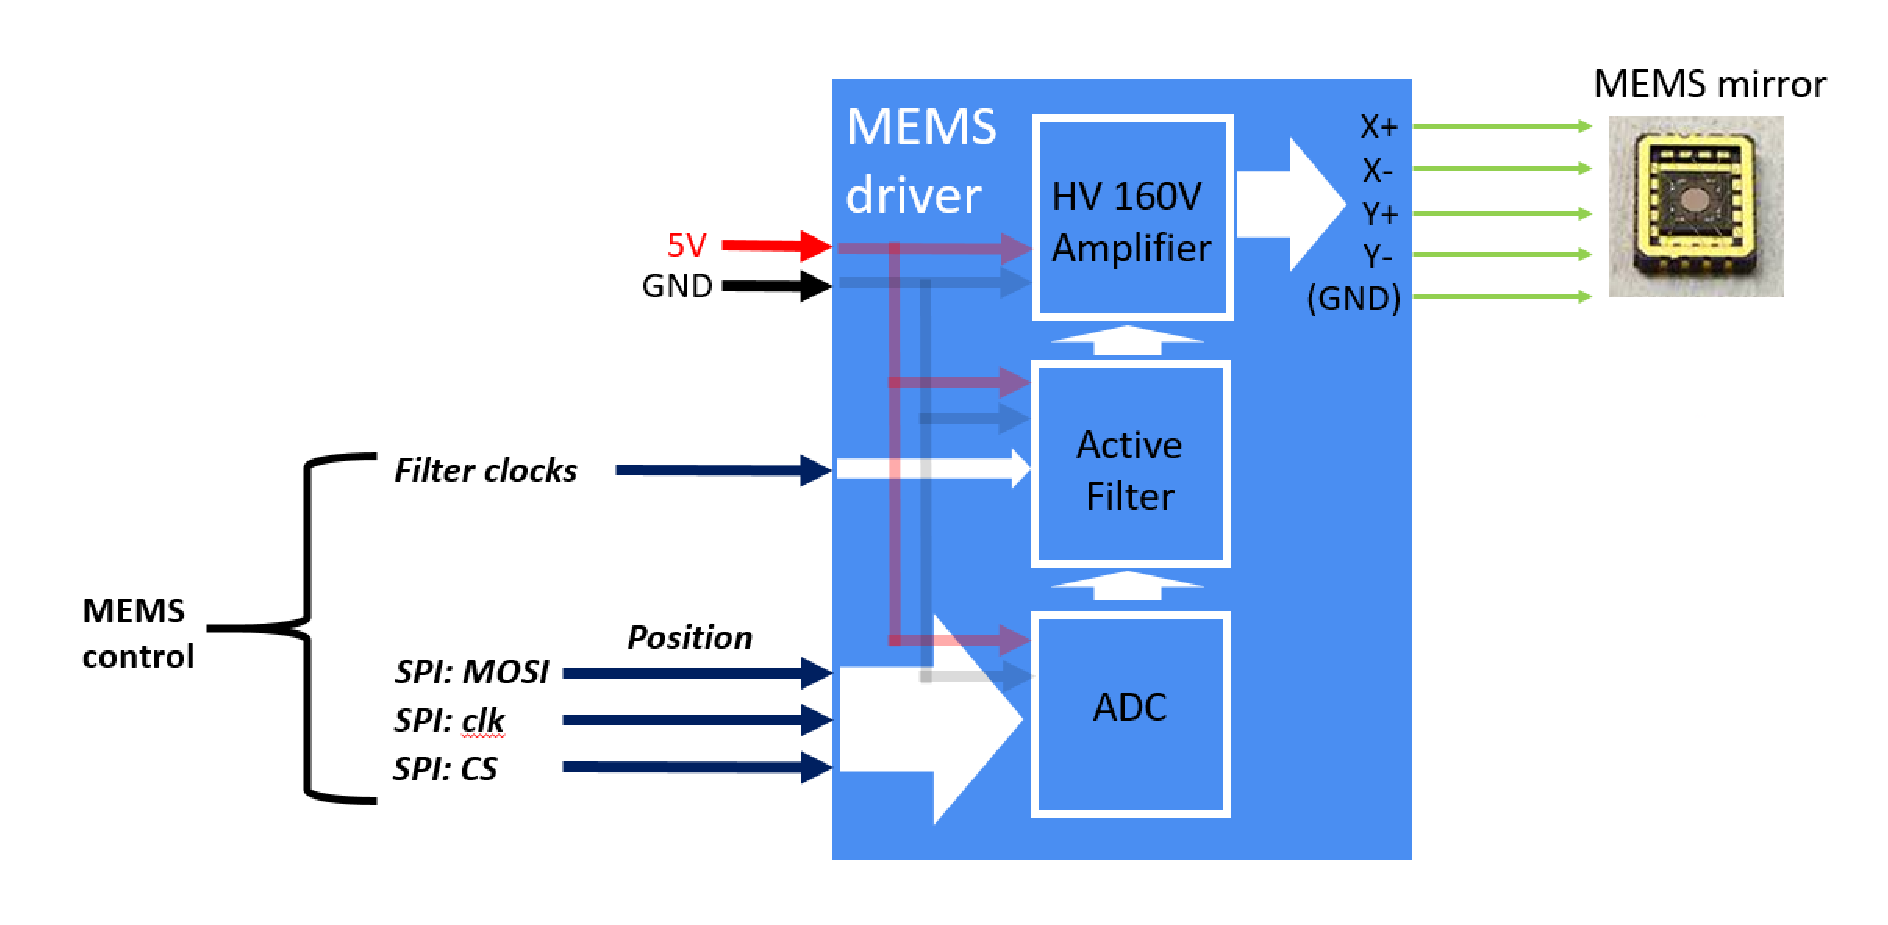
\includegraphics[width=1\linewidth]{mems_logic}
\caption{Logic diagram of MEMS driver.}
\label{fig:real_submodule}
\end{figure}


To form a trajectory with maximum possible FPS, for axis X applied voltage sine and for axis Y applied voltage like pulse with triangle shape. Depending on sine frequency we can get different number of lines, that makes vertical resolution very flexible as shiown in figure \ref{fig:mems_real_trajectories}.



\begin{figure}[H]
\includegraphics[width=1\linewidth]{mems_real_trajectories}
\caption{Photo of different resolutions: 4,8 and 60 lines.}
\label{fig:mems_real_trajectories}
\end{figure}





\subsection{SiPM logic}

SiPM board has a power (+5V) which is transformed to +29V for SiPM bias voltage and $\pm5 V$ for amplifier voltage. Readout contol (SPI) input are used for the control of TDC.
After aplification of the SiPM output (Fast out), signal goes to comparator, if level exceeds treshold, LH is provided to TDC Stop input.
After that, when TDC finished time calculation, Interrupt pin is fired and the result can be read by SPI DOUT.
Ref clk input is waiting for high frequecy clock signal - 12.5 MHz in our case, which is used for TDC measurement.



\begin{figure}[H]
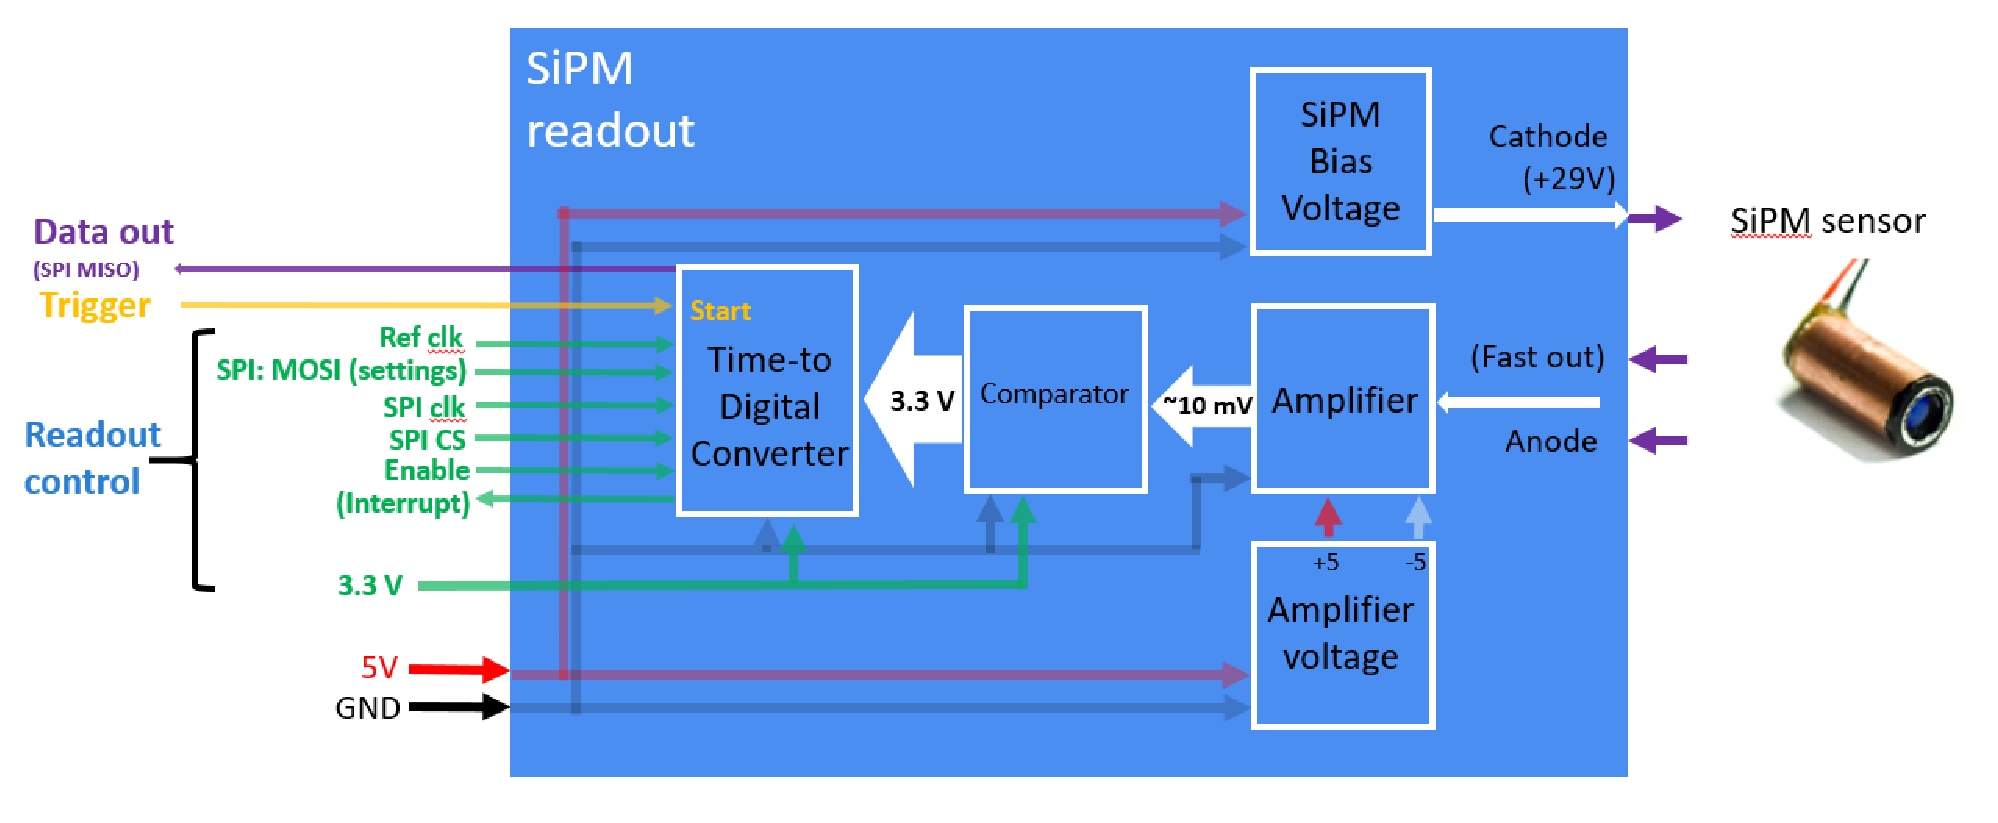
\includegraphics[width=1\linewidth]{sipm_logic}
\caption{Designed and real assembled submodule.}
\label{fig:real_submodule}
\end{figure}


During descring green board also desribe power board

\section{Control board}
In the beginning, logic control was performed by the micro CPU, which allowed to quickly develop a pilot version of the control board. Then, with growing needs, it became obvious the need to use FPGA, giving advantages in speed and parallelism, so the final version of the control board was completely implemented on FPGA.

The clock was modified via PLL from 50 to 64 MHz.
FPGA has faster clock + allow parallel \& less jitter.

\begin{figure}[H]
\includegraphics[width=1.1\linewidth]{control}
\caption{Designed and real assembled submodule.}
\label{fig:real_submodule}
\end{figure}
